\section{Methods}
\label{sec:method}

LaDiM uses dependencies between training computations to guide the investigation of a translated program. Starting from the Translator's candidate, the Verifier Agent examines the observed discrepancies and tests the code that could explain them. Its findings and supporting observations pass to a separate Repair Agent, which uses this evidence to select and evaluate changes. The Orchestrator returns measurements after each submission, allowing repair to follow the errors revealed as execution progresses. Figure~\ref{fig:architecture} shows this process.

\begin{figure}[!htb]
\centering
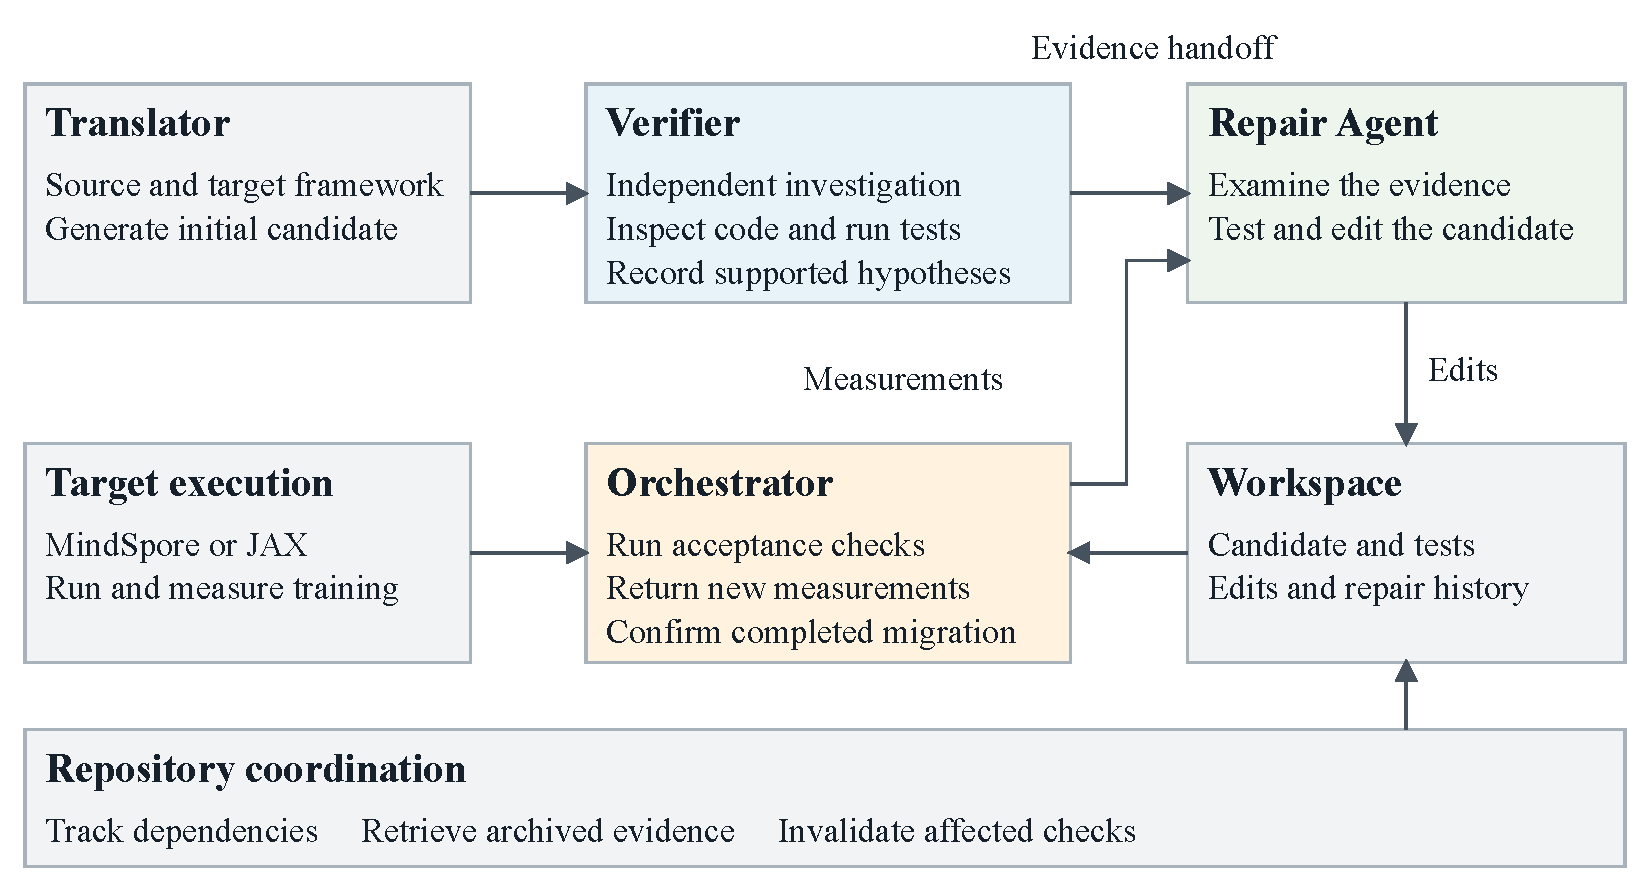
\includegraphics[width=\textwidth]{figures/hierarchical_feedback_architecture.pdf}
\caption{LaDiM's migration workflow. The Translator generates a candidate for the Verifier Agent to investigate through code and training observations. The Repair Agent receives the evidence and revises the candidate. The Orchestrator checks submitted changes and returns measurements for subsequent attempts. Execution adapters obtain observations from the target framework.}
\label{fig:architecture}
\end{figure}

\subsection{Preliminary}

A migration task $\mathcal T=(P,L_s,F_s,L_t,F_t,W)$ specifies a source program $P$, its language and framework $(L_s,F_s)$, the requested target environment $(L_t,F_t)$, and an editable file scope $W$. Migration produces a target program $\hat P$ that preserves the source's training behavior. An edit is one successfully applied editing operation, which can replace several code blocks across files in $W$. A submission follows a repair stage containing code inspection, tests, and edits.

At training step $t$, source and target executions produce corresponding observations $(e_t,v_t,g_t,\theta_{t+1}-\theta_t)$ and $(\hat e_t,\hat v_t,\hat g_t,\hat\theta_{t+1}-\hat\theta_t)$. Here $e_t$ records the execution outcome, including success or an exception, $v_t$ contains selected forward values and losses, $g_t$ contains gradients, and $\theta_t$ denotes the parameters before the update. After aligning corresponding tensors and parameters, we define
\begin{align}
d_{\mathrm{execution},t}&=\mathbf{1}[e_t\ne\hat e_t], &
d_{\mathrm{forward},t}&=v_t-\hat v_t,\\
d_{\mathrm{gradient},t}&=g_t-\hat g_t, &
d_{\mathrm{update},t}&=(\theta_{t+1}-\theta_t)-(\hat\theta_{t+1}-\hat\theta_t).
\end{align}
For a numerical comparison $d=x-\hat x$, $d\simeq0$ denotes agreement within its tolerance, such as $|d_j|\leq\alpha+\beta|x_j|$ for absolute tolerance $\alpha$ and relative tolerance $\beta$, or a specified norm bound. These discrepancies follow the training computation. Forward values determine the loss, differentiation produces the gradients, and the optimizer uses those gradients and its state to update parameters. The updated parameters then affect subsequent forward computations.

The LLM $M$ performs translation, investigation, and repair under the role instructions $A_T$, $A_V$, and $A_R$, respectively. The Orchestrator $\mathcal O$ evaluates candidates and manages the shared investigation and repair budget $B$. In the algorithms, $S$ holds the current candidate and observations, $H$ is a conversation, and $C$ manages retained evidence, preserving the conversation for individual programs and coordinating context for repositories. Each $\textsc{Query}(M,A,H,b,B)$ invokes $M$ with role instructions $A$ and conversation $H$, charging its usage to the stage allowance $b$ and shared budget $B$. The initial $\textsc{Translate}(M,A_T,\mathcal T)$ call uses the same LLM to generate a candidate. Tools return observations and update $S$ when an edit succeeds.

\subsection{Verifier Agent: Layered Diagnosis}
\label{sec:hierarchy}

The Verifier Agent uses the dependencies between discrepancies to select code and tests for investigation. For an \textbf{execution discrepancy} ($d_{\mathrm{execution},t}=1$), the Verifier examines the exception and implicated calls and constructs a focused reproduction. For a \textbf{forward discrepancy} ($d_{\mathrm{forward},t}\not\simeq0$), it traces the operators producing different values and tests whether the same error explains downstream differences. When $d_{\mathrm{forward},t}\simeq0$, a \textbf{gradient discrepancy} ($d_{\mathrm{gradient},t}\not\simeq0$) directs attention to parameter registration and the differentiation path. For example, inspecting a parameter's registration and tracing its connection to the loss can distinguish an unregistered parameter from a disconnected computation. When $d_{\mathrm{forward},t}\simeq0$ and $d_{\mathrm{gradient},t}\simeq0$, an \textbf{update discrepancy} ($d_{\mathrm{update},t}\not\simeq0$) motivates inspection of the optimizer's rule and state. The first affected step also guides investigation because updates influence later forward values. Algorithm~\ref{alg:diagnose} records the agent's observations, tool calls, and conclusions as evidence for repair.

\begin{algorithm}[!htb]
\caption{\textsc{Investigate}$(\mathcal T,S,M,B,C)$}
\label{alg:diagnose}
\begin{algorithmic}[1]
\Require Task $\mathcal T$, candidate and discrepancies in $S$, LLM $M$, budget $B$, context $C$
\Ensure Verifier investigation $E$
\State $H\gets\Call{StartConversation}{A_V,\mathcal T,S}$; $b\gets\Call{DiagnosisAllowance}{B}$
\While{$\Call{WithinLimits}{b,B}$}
  \State $H\gets C.\Call{BeforeCall}{H,S}$; $a\gets\Call{Query}{M,A_V,H,b,B}$
  \State $H\gets H\mathbin{\|}a$
  \If{$a.\mathrm{complete}$} \State \Return $\Call{PublicEvidence}{H,C.\mathrm{archive}}$ \EndIf
  \ForAll{$c\in a.\mathrm{toolCalls}$}
    \State $r\gets\Call{Execute}{c,S,\mathrm{productionReadOnly}=\mathrm{true}}$
    \State $H\gets H\mathbin{\|}(c,r)$; $C.\Call{Record}{c,r,S}$
  \EndFor
\EndWhile
\State \Return $\Call{PublicEvidence}{H,C.\mathrm{archive}}$
\end{algorithmic}
\end{algorithm}

\subsection{Repair Agent: Evidence Handoff}

The Repair Agent begins a separate conversation with the Verifier Agent's recorded investigation, including code observations, test results, and final diagnosis. These records are attributed to the Verifier Agent, allowing the Repair Agent to reassess a hypothesis and choose further tests before editing. The Repair Agent retains the inspection and testing tools and can modify files in $W$. It continues until it has applied and tested a change and returns its report, or exhausts the stage allowance. The stage flags $F$ track successful production edits and tests performed after the latest edit. After each submission, the Orchestrator returns new measurements. Comparing them with earlier observations reveals which differences the edit resolved and which computations warrant further investigation. The candidate and repair conversation persist across attempts under one cumulative budget. Algorithm~\ref{alg:repair} also confirms candidates that already pass after investigation, allowing them to finish without corrective edits.

\begin{algorithm}[!htb]
\caption{\textsc{Repair}$(\mathcal T,S,M,B,C)$}
\label{alg:repair}
\begin{algorithmic}[1]
\Require Task $\mathcal T$, candidate state $S$, LLM $M$, budget $B$, context $C$
\Ensure Current candidate and verification status
\State \textbf{if} $S.m=\varnothing$ \textbf{then} $S.m\gets\mathcal O.\Call{Measure}{S.\hat P}$
\State $E\gets\Call{Investigate}{\mathcal T,S,M,B,C}$
\State $(S.m,q)\gets\mathcal O.\Call{Verify}{S.\hat P}$
\If{$q=\mathrm{accepted}$} \State \Return $(S.\hat P,q)$ \EndIf
\State $H\gets\Call{StartConversation}{A_R,\mathcal T,\operatorname{AttributeToVerifier}(E)}$
\State $C.\mathrm{handoff}\gets\mathrm{true}$
\While{$\Call{SubmissionsLeft}{B}\land\Call{BudgetLeft}{B}$}
  \State $H\gets H\mathbin{\|}S.m$; $F\gets(\mathrm{edited}=\mathrm{false},\mathrm{tested}=\mathrm{false})$
  \State $b\gets\Call{RepairAllowance}{B}$
  \While{$\Call{WithinLimits}{b,B}$}
    \State $H\gets C.\Call{BeforeCall}{H,S}$; $a\gets\Call{Query}{M,A_R,H,b,B}$
    \State $H\gets H\mathbin{\|}a$
    \If{$\Call{ReadyToSubmit}{a,F}$} \State \textbf{break} \EndIf
    \ForAll{$c\in a.\mathrm{toolCalls}$}
      \State $r\gets\Call{Execute}{c,S,\mathrm{editableScope}=W}$; $F\gets\Call{UpdateFlags}{F,c,r}$
      \State $H\gets H\mathbin{\|}(c,r)$; $C.\Call{Record}{c,r,S}$
    \EndFor
  \EndWhile
  \State $(S.m,q)\gets\mathcal O.\Call{Verify}{S.\hat P}$; $B.\mathrm{submissions}\gets B.\mathrm{submissions}+1$
  \If{$q=\mathrm{accepted}$} \State \Return $(S.\hat P,q)$ \EndIf
\EndWhile
\State \Return $(S.\hat P,q)$
\end{algorithmic}
\end{algorithm}

\subsection{Repository Coordination}
\label{sec:repository-method}

A change to a shared implementation can affect several callers in a repository. LaDiM provides a map of files, imports, symbols, and notebook cells from which the agent proposes work units with file scopes, interface goals, and dependencies. It selects a unit whose prerequisites have current checkpoints, then investigates the related interfaces. Checkpoints record syntax validation and selected local tests. Code changes invalidate checkpoints for affected units and their dependents, prompting checks of the callers that may have changed behavior. The Orchestrator evaluates the complete repository, including its entry points and training computations, to determine acceptance.

Repository context management carries relevant evidence as investigation moves across files. LaDiM archives observations and conversations and provides a tool for retrieving detailed records. At the role handoff, an actual switch between work units, or a context capacity boundary, it rebuilds the conversation around the current plan, hypotheses, measurements, and relevant code already inspected. Earlier measurements retain their association with the candidate on which they were obtained. Algorithm~\ref{alg:repository} supplies these context operations to Algorithms~\ref{alg:diagnose} and~\ref{alg:repair}.

\begin{algorithm}[!htb]
\caption{Repository migration and context operations}
\label{alg:repository}
\begin{algorithmic}[1]
\Function{RepositoryMigrate}{$\mathcal T,M,B$}
  \State $S.\hat P\gets\Call{Translate}{M,A_T,\mathcal T}$; $C\gets\Call{RepositoryContext}{\operatorname{Map}(\mathcal T)}$
  \State $(S.m,q)\gets\mathcal O.\Call{Verify}{S.\hat P}$
  \If{$q=\mathrm{accepted}$} \State \Return $(S.\hat P,q)$ \EndIf
  \State \Return $\Call{Repair}{\mathcal T,S,M,B,C}$
\EndFunction
\Function{$C$.Record}{$c,r,S$}
  \State $C.\mathrm{archive}\gets C.\mathrm{archive}\mathbin{\|}(c,r)$
  \If{$\Call{CodeChanged}{r}$}
    \State $\Call{MarkHistorical}{C.\mathrm{measurements}}$
    \State $\Call{Invalidate}{C.\mathrm{checkpoints},\operatorname{AffectedUnitsAndDependents}(r,C.\mathrm{plan})}$
  \EndIf
  \State $(C.\mathrm{plan},C.\mathrm{unit},C.\mathrm{checkpoints})\gets\Call{Update}{c,r,C}$
\EndFunction
\Function{$C$.BeforeCall}{$H,S$}
  \If{$C.\mathrm{handoff}\lor\Call{UnitSwitched}{C}\lor\Call{AtCapacity}{H}$}
    \State $\Call{Archive}{C,H}$
    \State $K\gets\Call{CurrentReadCode}{C.\mathrm{unit},S.\hat P}$
    \State $E\gets\Call{PublicFindings}{H,C.\mathrm{archive}}$
    \State $H\gets\Call{Rebuild}{H.\mathrm{role},C.\mathrm{plan},E,S.m,K}$
    \State $C.\mathrm{handoff}\gets\mathrm{false}$; $C.\mathrm{previousUnit}\gets C.\mathrm{unit}$
  \EndIf
  \State \Return $H$
\EndFunction
\end{algorithmic}
\end{algorithm}
